% TEMPLATE for Usenix papers, specifically to meet requirements of
%  USENIX '05
% originally a template for producing IEEE-format articles using LaTeX.
%   written by Matthew Ward, CS Department, Worcester Polytechnic Institute.
% adapted by David Beazley for his excellent SWIG paper in Proceedings,
%   Tcl 96
% turned into a smartass generic template by De Clarke, with thanks to
%   both the above pioneers
% use at your own risk.  Complaints to /dev/null.
% make it two column with no page numbering, default is 10 point

% Munged by Fred Douglis <douglis@research.att.com> 10/97 to separate
% the .sty file from the LaTeX source template, so that people can
% more easily include the .sty file into an existing document.  Also
% changed to more closely follow the style guidelines as represented
\section{Evaluation} \label{sec:eva}
%
We have implemented the proposed prototype demonstrated in previous sections. The implementation added or changed %$350$ SLoC to Linux kernel and $166$ SLoc to Xen hypervisor, of which $2$ SLoc in the hypervisor are
$166$ SLoc of Xen hypervisor and $350$ SLoC of Linux kernel.
This section evaluates the performance of \name by running both micro- and macro-benchmark kits.

\subsection{Experimental Setup}

Our experimental platform is a LENOVO QiTianM4390 PC with Intel Core i5-3470 running at 3.20 GHz, four CPU cores available to the system. We enable the Intel VT-d feature in the BIOS menu, which supports queue-based invalidation interface in the granularity of page invalidation. Xen version 4.2.1 is used as the hypervisor while \emph{domain 0} uses the Ubuntu version 12.04 and kernel version 3.2.0. Besides, \emph{domain 0} configures its grub.conf to enable DMA address translation mode of IOMMU and to print log information to a serial port in debug mode.

In the original design of Xen, page table (de)allocations will give rise to page type updates, upon which the function iotlb\_flush\_qi will be invoked to flush corresponding IOTLB entries. Thus, a global counter is placed into the function body to record invocation times of the function and then an average counter per minute is calculated as a frequency of IOTLB-flush. When the IOTLB-flush stays at zero level, it means that no page table is (de)allocated, indicating that no process creation/exit occurs then. In a nutshell, there exists a mutually positive effect between a process creation/exit and IOTLB-flush.

Because of that, we define two different system states, classified by the frequency of IOTLB-flush.

\emph{idle state}: When the system boots up and logins into the graphical desktop, lots of system processes are created, causing many IOTLB flushes. But as time goes by, the frequency of IOTLB-flush reduces rapidly and stays stable to zero level ten minutes later, and we think that system starts to be in an \emph{idle state}, where no new process creation/exit does occur while existing system daemons are still running.

\emph{busy state}: A stress tool emulating a concurrent-processes workload is developed to make the system become \emph{busy}. Specifically, the tool is busy periodically launching a default browser(e.g., Mozilla Firefox 31.0 in the experiment), opening new tabs one by one and then closing the browser gracefully in an infinite loop, so as to constantly create/terminate a large number of Firefox processes, thus giving rise to frequent page type updates of page tables. More specifically, one iteration of the loop costs five minutes and the frequencies of process creation and exit are $542.14$ times per minute and $542.07$ times per minute, respectively. Besides, the memory usage of the tool on an average iteration is $284.1$ MB. Please note that since the frequency of IOTLB-flush will become stable five minutes after the tool is launched, time period of one iteration is also set to that interval to achieve a stable frequency of IOTLB-flush.

Both micro- and macro-benchmark kits are performed under the \emph{busy state}, in which micro tests are utilized to evaluate the frequency of IOTLB-flush, CPU usage and memory size while macro-benchmarks give an assessment on overall system performance.

\subsection{Micro-Benchmarks}

Micro-experiments are conducted in three groups. In a baseline group, the \emph{idle} system enters into the \emph{busy state} under Xen's original design. On the contrary, in a pre-\name group, \name is enabled before system becomes \emph{busy}. Besides, in another group of dyn-\name, \name is dynamically enabled (e.g., five minutes after the tool is invoked) so as to evaluate the performance of dyn-\name compared to the other groups.

\begin{figure}[ht]
\centering
%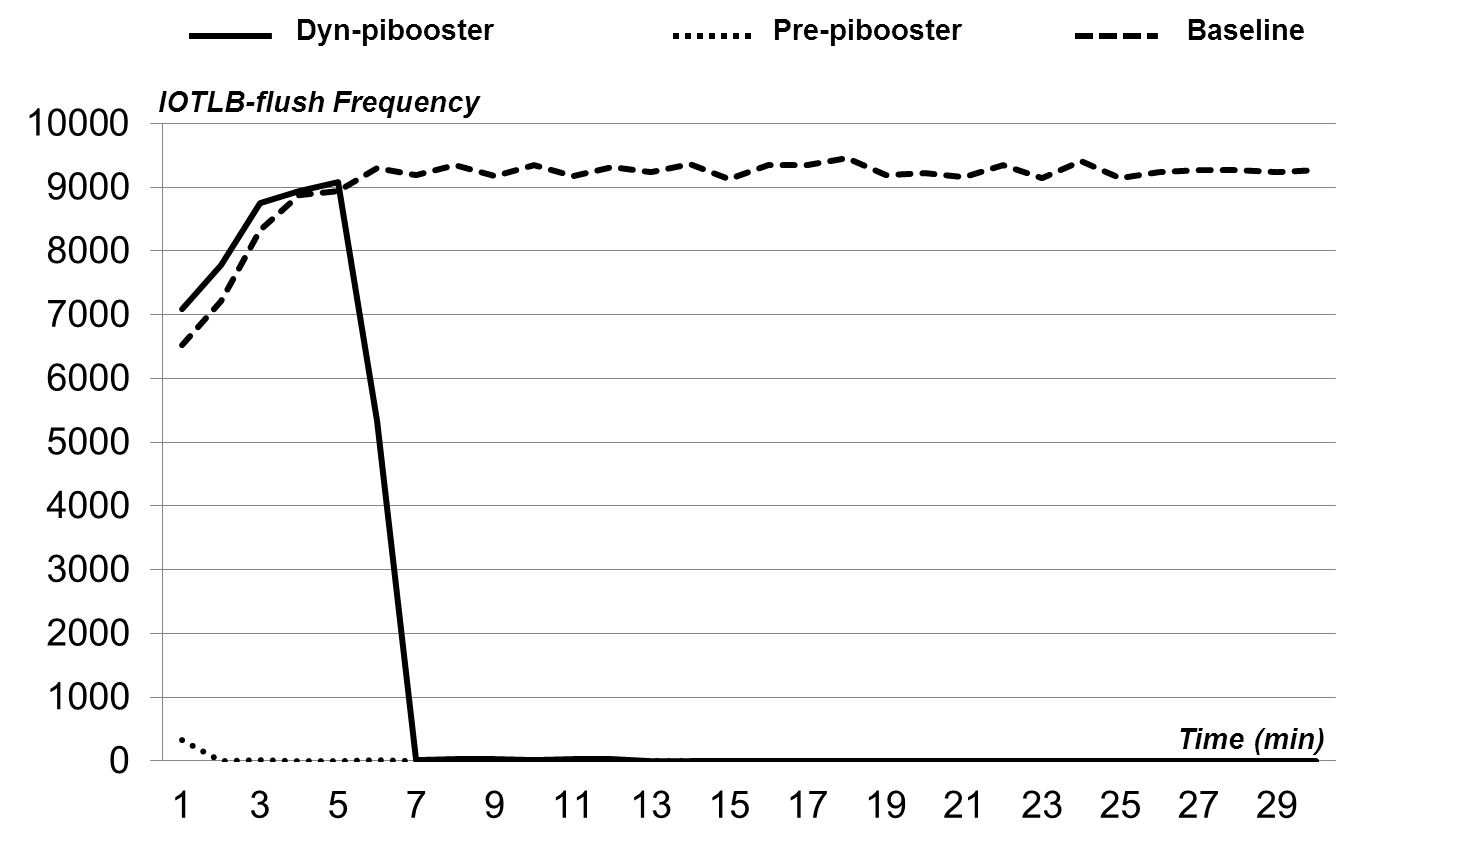
\includegraphics[scale=0.55]{image/iotlbflush.png} \\
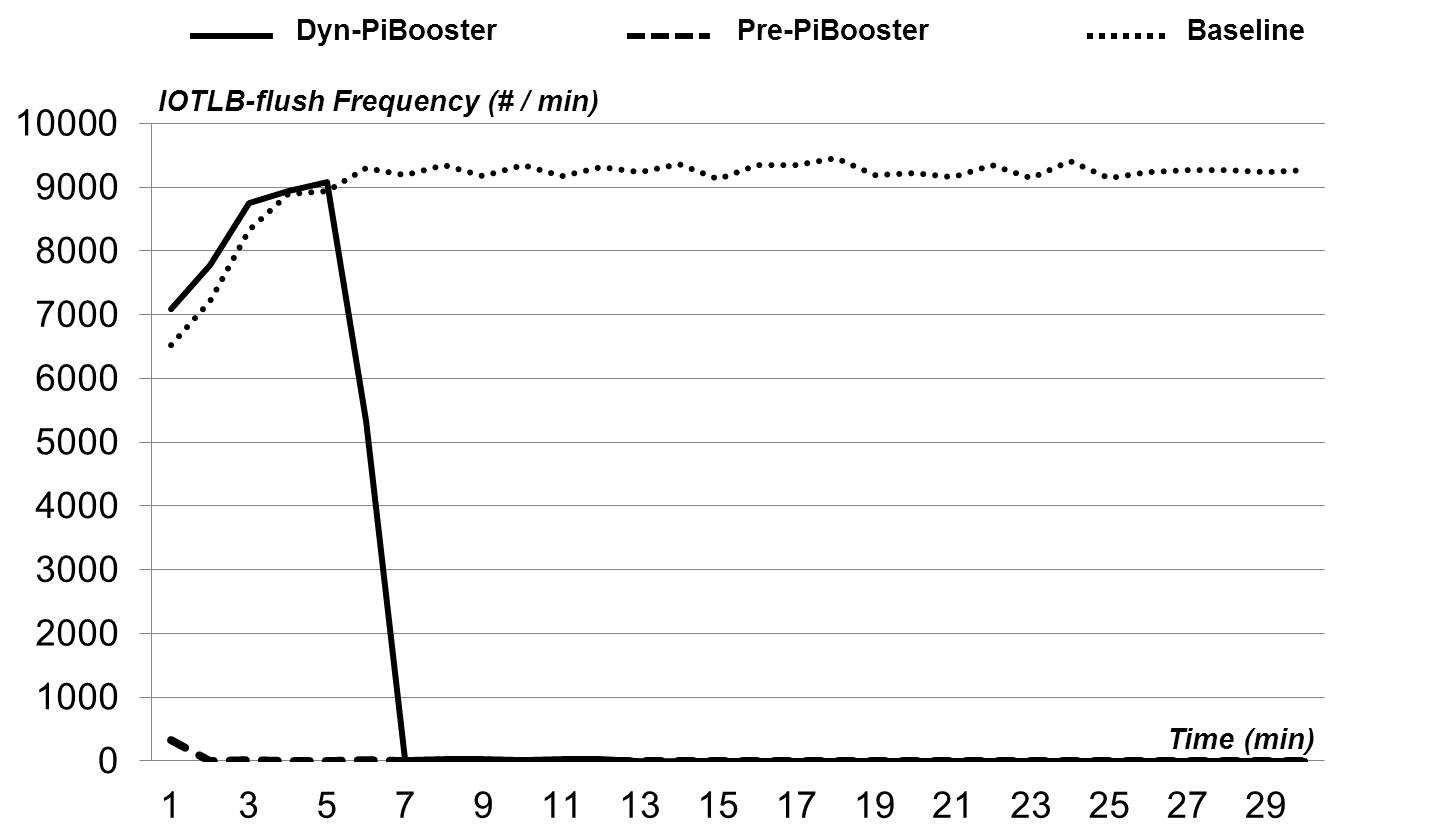
\includegraphics[width=0.5\textwidth]{image/micro/iotlbflush.jpg} \\
\caption{Frequency of IOTLB-flush in the pre-\name group is reduced to zero within one minute. If \name is dynamically enabled when IOTLB is flushing frequently, the frequency drops sharply within two minutes from the high level to zero and remains unchanged since then, contrary to that of the baseline group.}
\label{fig:iotlbflush}
\end{figure}

As can be seen from Figure~\ref{fig:iotlbflush}. Y-axis represents the frequency of IOTLB-flush, corresponding to the time period (i.e., one minute) of x-axis for the first thirty minutes that the \emph{busy state} lasts. From this figure, frequency in the baseline group increases rapidly and remains stable five minutes later. By contrast, frequency in the pre-\name group drops to zero level in a very short time. It can be safely concluded that the fine-grained validation module proposed by \name does eliminate the IOTLB flushes caused by concurrent processes creations/exits. The dyn-\name group shows that the frequency also can be dropped to zero level very quickly even if the system is already in a \emph{busy state}.

\begin{figure*}[t!]
    \centering
    \begin{subfigure}[t]{0.5\textwidth}
        \centering
        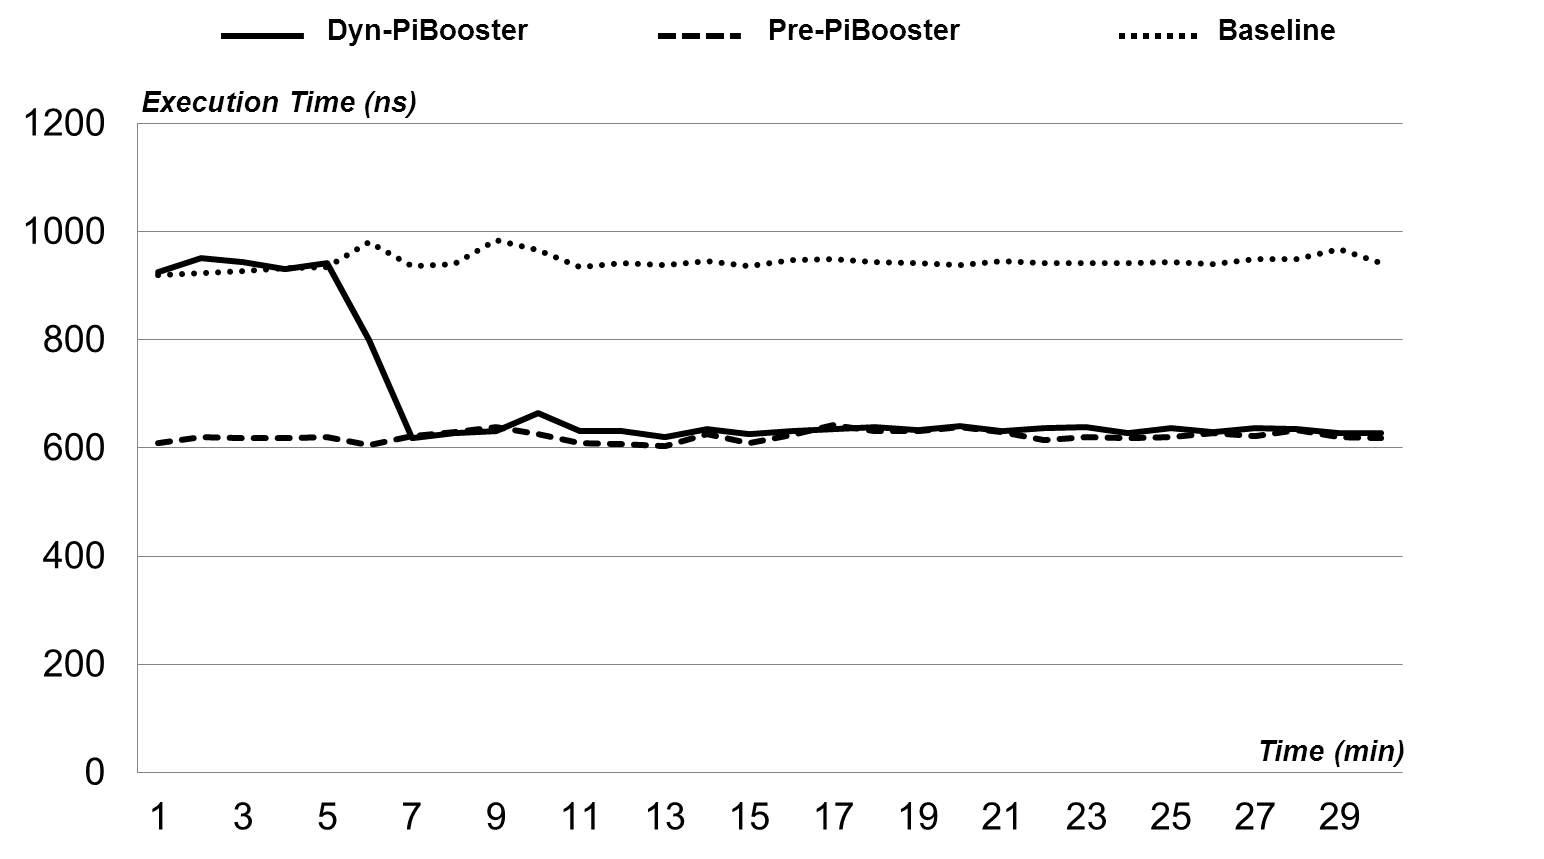
\includegraphics[height=2.0in]{image/micro/PGDalloc.png}
        \caption{Execution time of pgd\_alloc}
        \label{fig:subfig:a}
    \end{subfigure}%
    ~
    \begin{subfigure}[t]{0.5\textwidth}
        \centering
        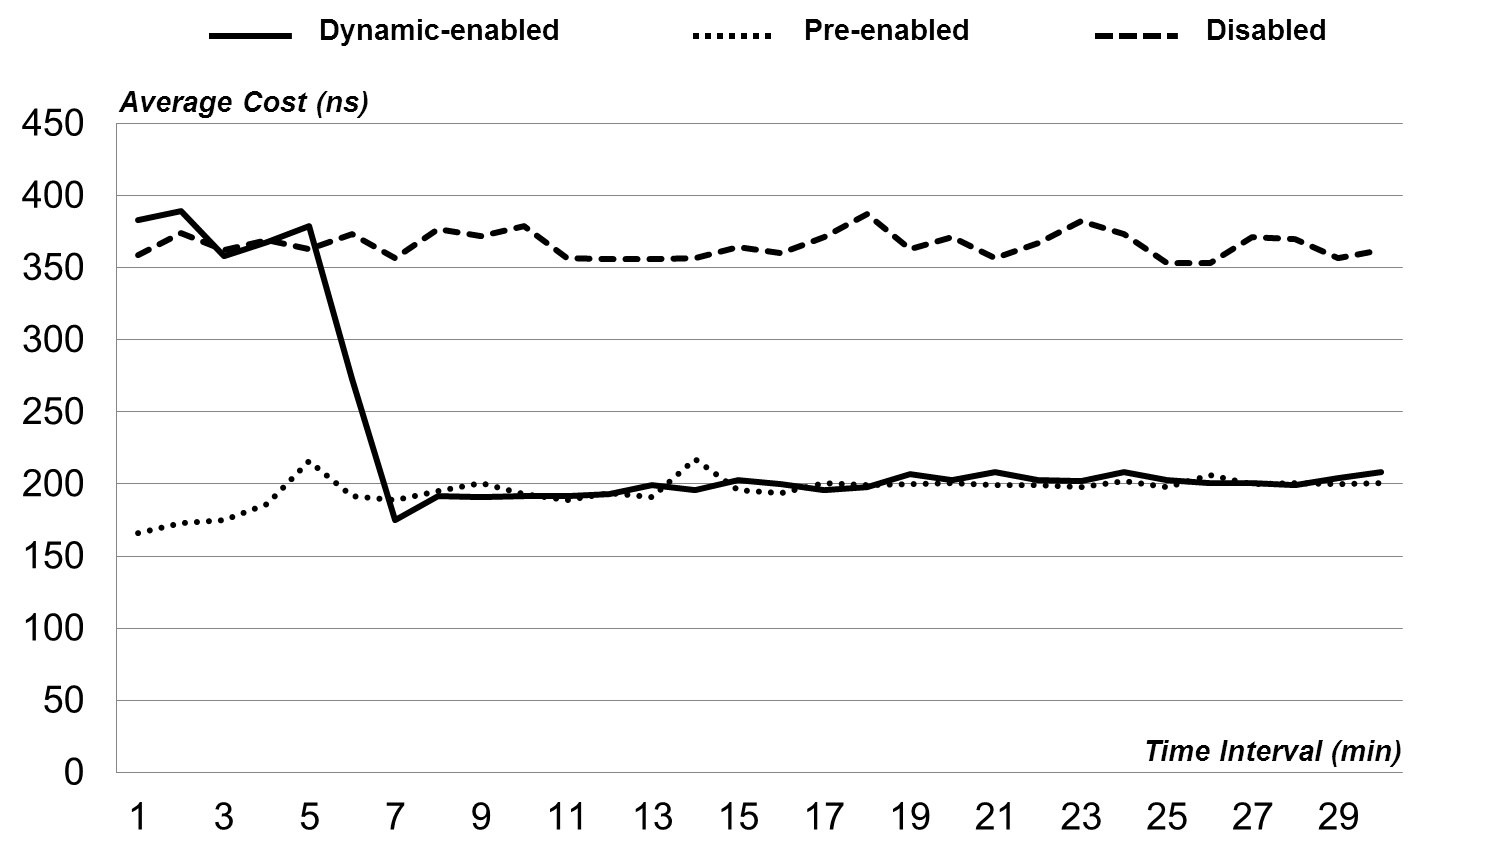
\includegraphics[height=2.0in]{image/micro/PGDfree.png}
        \caption{Execution time of pgd\_free}
        \label{fig:subfig:b}
    \end{subfigure}
    \caption{The time cost in the dyn-\name group is reduced quickly within two minutes to the low level as pre-\name group maintains. And the total execution time of both functions in the pre-\name group is reduced by xx\% compared to that of the baseline group.}
    \label{fig:PGDtime}
\end{figure*}

\begin{figure*}[t!]
    \centering
    \begin{subfigure}[t]{0.5\textwidth}
        \centering
        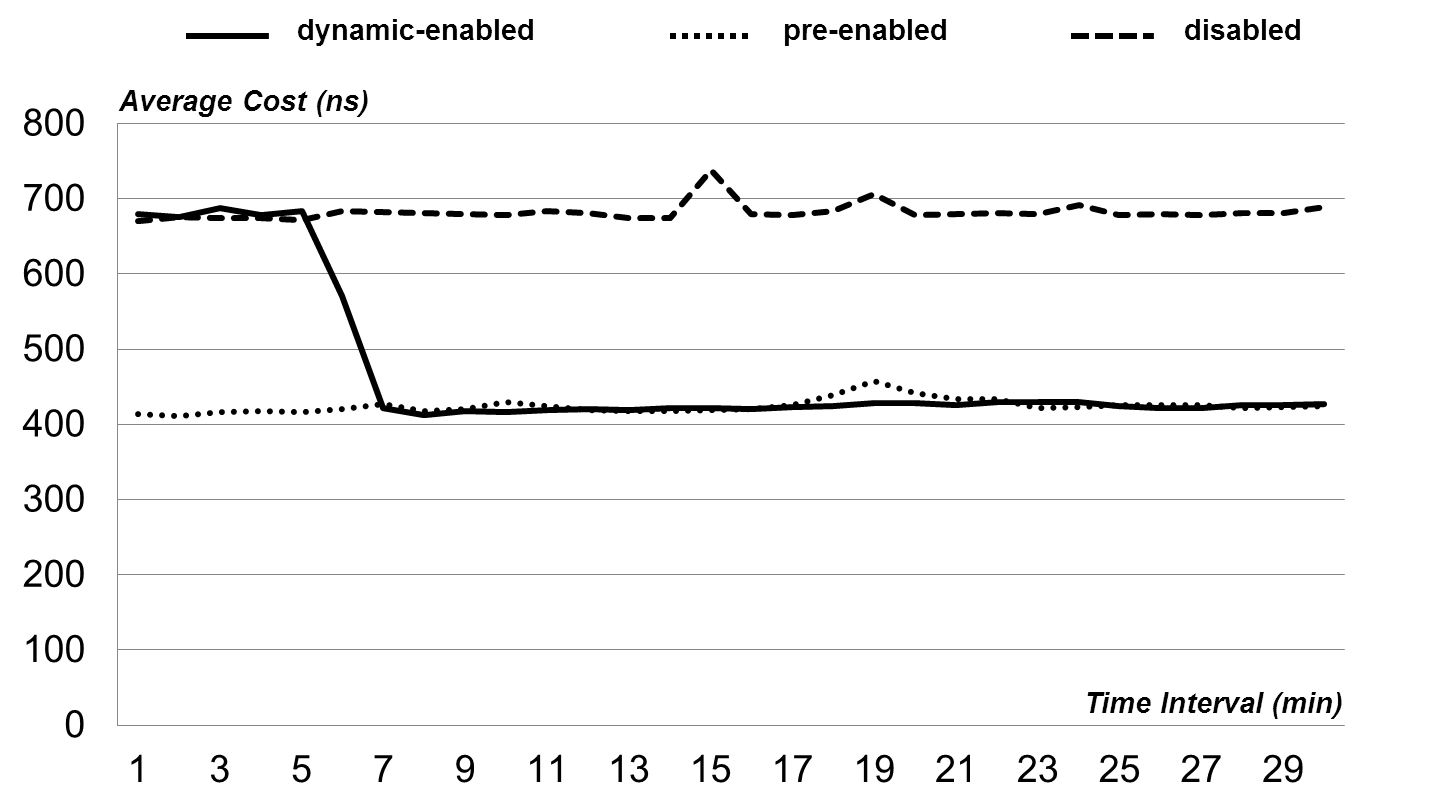
\includegraphics[height=2.0in]{image/micro/PMDalloc.png}
        \caption{Execution time of pmd\_alloc}
        \label{fig:subfig:a}
    \end{subfigure}%
    ~
    \begin{subfigure}[t]{0.5\textwidth}
        \centering
        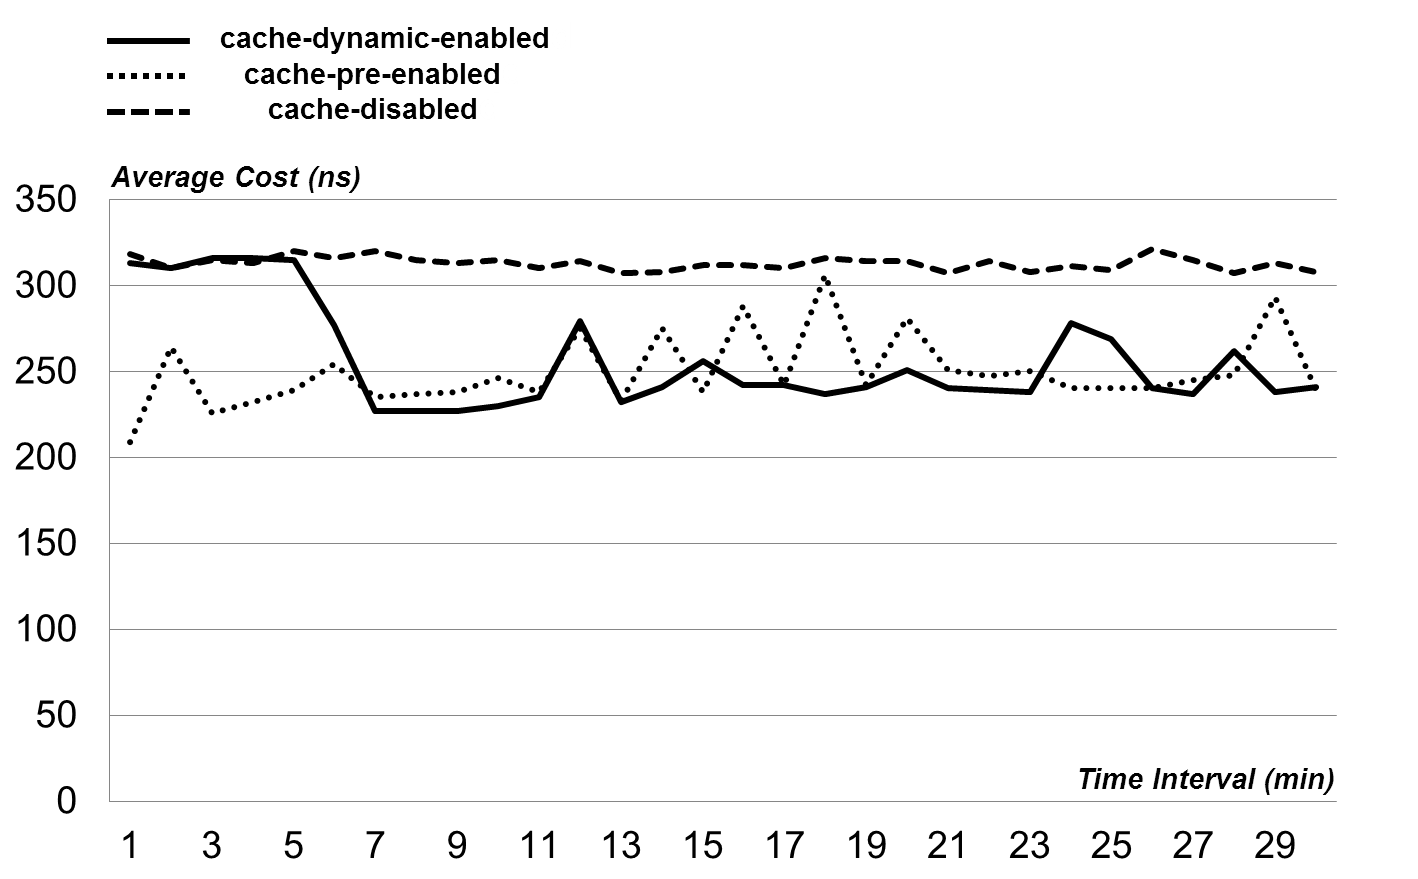
\includegraphics[height=2.0in]{image/micro/PMDfree.png}
        \caption{Execution time of pmd\_free}
        \label{fig:subfig:b}
    \end{subfigure}
    \caption{The trend of time cost in the dyn-\name group behaves like Figure~\cite{fig:PGDtime}. And the total execution time of both functions in the pre-\name group is reduced by xx\% compared to that of the baseline group.}
    \label{fig:PMDtime}
\end{figure*}

\begin{figure*}[t!]
    \centering
    \begin{subfigure}[t]{0.5\textwidth}
        \centering
        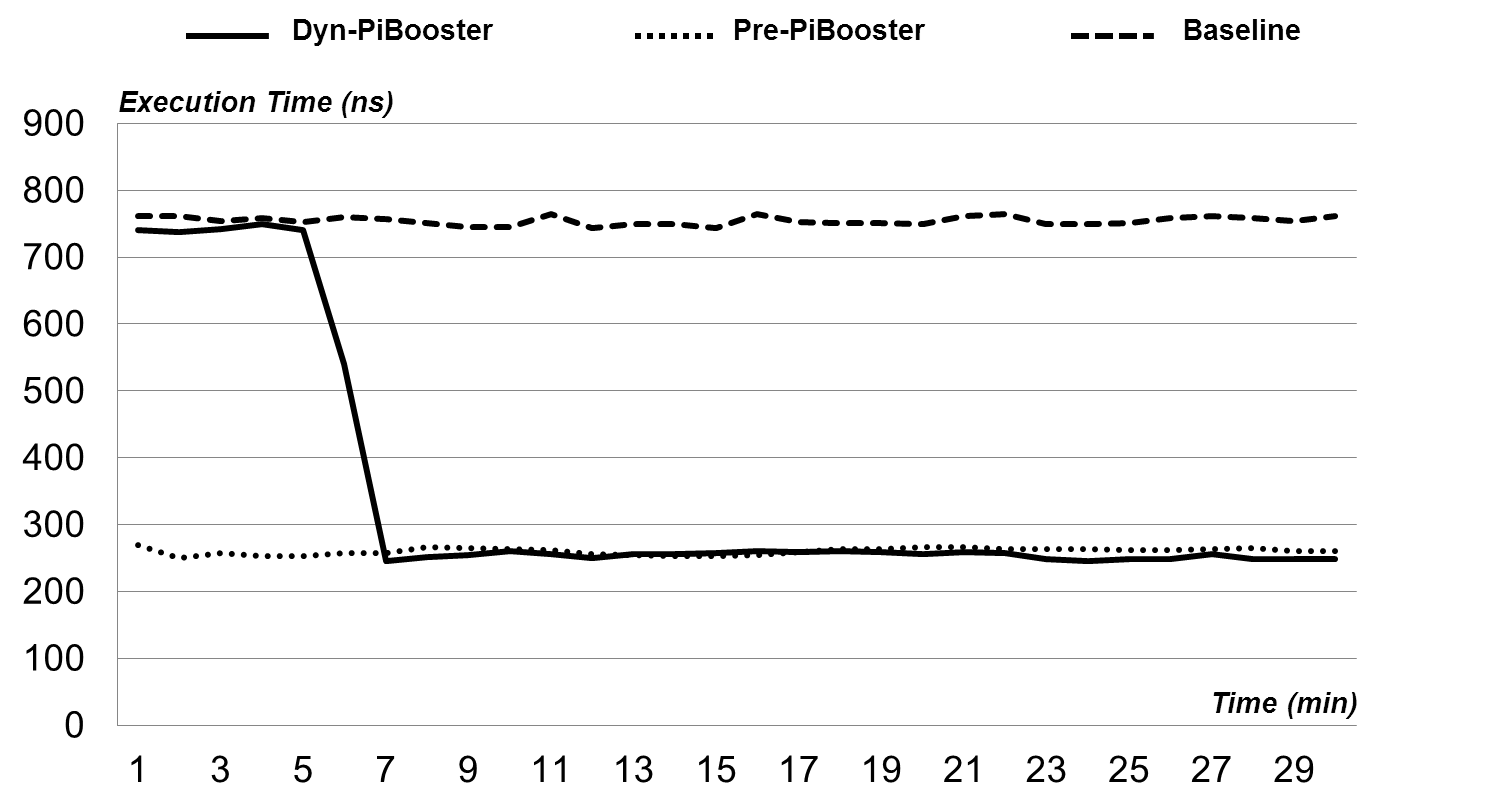
\includegraphics[height=2.0in]{image/micro/PTEalloc.png}
        \caption{Execution time of pte\_alloc}
        \label{fig:subfig:a}
    \end{subfigure}%
    ~
    \begin{subfigure}[t]{0.5\textwidth}
        \centering
        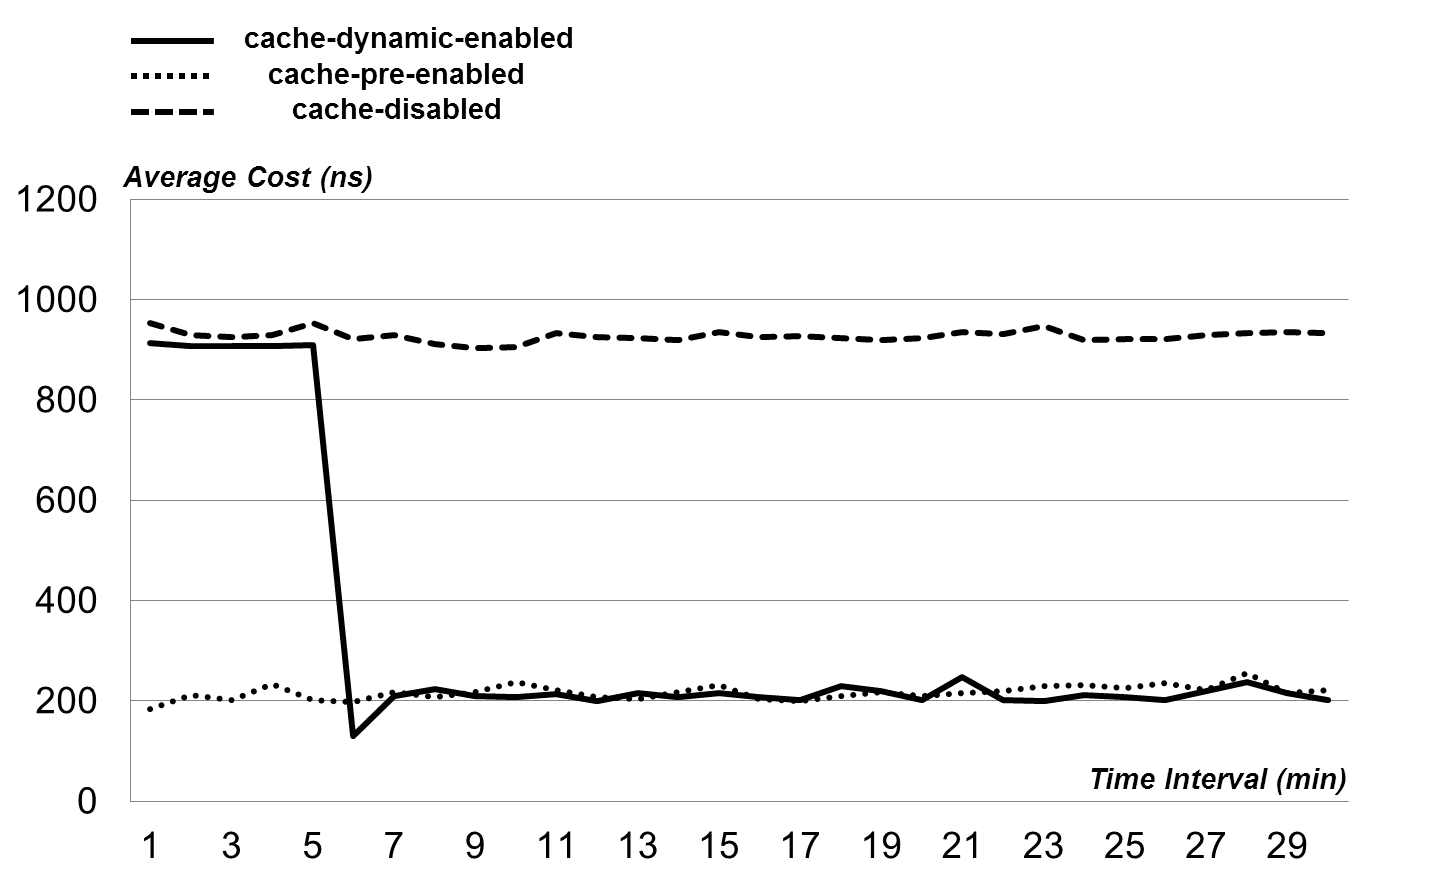
\includegraphics[height=2.0in]{image/micro/PTEfree.png}
        \caption{Execution time of pte\_free}
        \label{fig:subfig:b}
    \end{subfigure}
    \caption{The trend of time cost in the dyn-\name group behaves like Figure~\ref{fig:PGDtime} and \ref{fig:PMDtime}. And the total execution time of both functions in the pre-\name group is reduced by xx\% compared to that of the baseline group.}
    \label{fig:PTEtime}
\end{figure*}

Now let’s move to CPU time that every group will cost. Specifically, each level of page table has its (de)allocation functions, e.g., pgd\_alloc and pgd\_free, and the average execution time of each function is calculated per minute. As shown in Figure~ \ref{fig:PGDtime},\ref{fig:PMDtime},\ref{fig:PTEtime}, both allocation and deallocation functions in all levels of page table in the pre-\name group respectively consume 45\% less and 55\% less CPU time in nanoseconds on average, compared to that of the baseline group, indicating that \name has largely improved the performance of page table (de)allocations by maintaining a dedicated cache.

%When cache is pre-enabled, the ratio between the total pages in cache and the total pages as page tables is approximately equal to 1:1, which indicates that the cache mechanism takes up a small memory percentage of the stress tool.
\begin{table}[!ht]
\footnotesize
\begin{center}
\begin{tabular}{|l|l|l|}
\hline
{\textbf{Page-Table Type}} & {\textbf{Cache (Page \#)}} & {\textbf{Page Table (Page \#)}} \\ \hline
PGD & $5$  & $4$ \\ \hline
PMD & $26$ & $12$ \\ \hline
PTE & $145$ & $177$ \\ \hline
Total & $176$ & $193$ \\ \hline
\end{tabular}
\end{center}
\caption{In the pre-\name group, the ratio between the total cached pages in cache and the page table pages is approximately equal to 1:1 just as expected. And the memory size of cached pages only takes up to 0.2\% of the tool's memory.}
\label{tab:prePGpool}
\end{table}

\begin{table}[!ht]
\footnotesize
\begin{center}
\begin{tabular}{|l|l|l|}
\hline
{\textbf{Page-Table Type}} & {\textbf{Cache (Page \#)}} & {\textbf{Page Table (Page \#)}} \\ \hline
PGD & $4$  & $2$ \\ \hline
PMD & $20$ & $4$  \\ \hline
PTE & $136$ & $182$ \\ \hline
Total & $160$ & $188$ \\ \hline
\end{tabular}
\end{center}
\caption{In the dyn-\name group, the ratio between the total cached pages in cache and the page table pages is approximately equal to 1:1 as expected. And the memory size of cached pages only takes up to 0.2\% of the tool's memory.}
\label{tab:dynPGpool}
\end{table}

Besides CPU usage, \name is evaluated in the aspect of memory consumption. Cache size in the pre-\name group shown in Table \ref{tab:prePGpool} reaches only $176$ pages(i.e., ($176 * 4K$) $<$ $1$M) at most in the long time run, only 0.2\% percentage of the tool's memory (i.e., $284.1$ MB). Besides, memory size in Table \ref{tab:dynPGpool} shows that the dyn-\name group takes up is only $160$ pages at most, also a small percentage of the tool's memory. Both groups consume an insignificant memory usage and reach a satisfying tradeoff between CPU time and memory size. Also note that the conditions of freeing pages in cache in the dyn-\name group heavily rely on a specific scenario, which may not work for other situations. We will further discuss the conditions in future work.

%And the reason why the dyn-\name group has fewer cached pages than that of the pre-\name group is that a certain number of page table pages has been freed to the memory allocator before the \name is enabled.

\mypara{a worst case} As mentioned before, guest kernel firstly goes through \name cache to require enough semi-writable pages when page creations occur. If the cache cannot satisfy the requirements (a.k.a, cache miss), writable pages from the memory allocator will be allocated to corresponding process creations, and these pages will be validated by \name module. Since these pages are judged not to be semi-writable, Xen will enforce both software and DMA protections, which will produce the same number of IOTLB flushes as the baseline. As a result, the execution path of page table allocation in \name in this worst case is longer than that of the baseline. More precisely, \name executes four more instructions than the baseline, and they are two conditional statements, i.e., \name checks if the cache is NULL, \name checks whether the allocated page is semi-writable. Nevertheless, the worse case does not often occur in \name. According to our observations in the dyn-\name group, the probability of cache miss is only xx\% for the thirty minutes since \name is enabled, which indicates that \name performs much better than the baseline in the long-time run.
\zhi{In the pre-\name group, the probabilities of cache miss are 9/550 (1\% PGD), 38/2200(1\% PMD), 322/6633(4\% PTE),respectively. In the dyn-\name group, the probabilities of cache miss are 7/540 (1\% PGD), 24/2160(1\% PMD), 320/6333(5\% PTE),respectively.}


\subsection{Macro-Benchmarks}

Macro-benchmarks are made use of to evaluate the effects of \name on overall system performance. Since dyn-\name group does apply in real cases, macro tests are conducted in two groups, i.e., a baseline group and a dyn-\name group.

\begin{figure}[htp]
\centering
%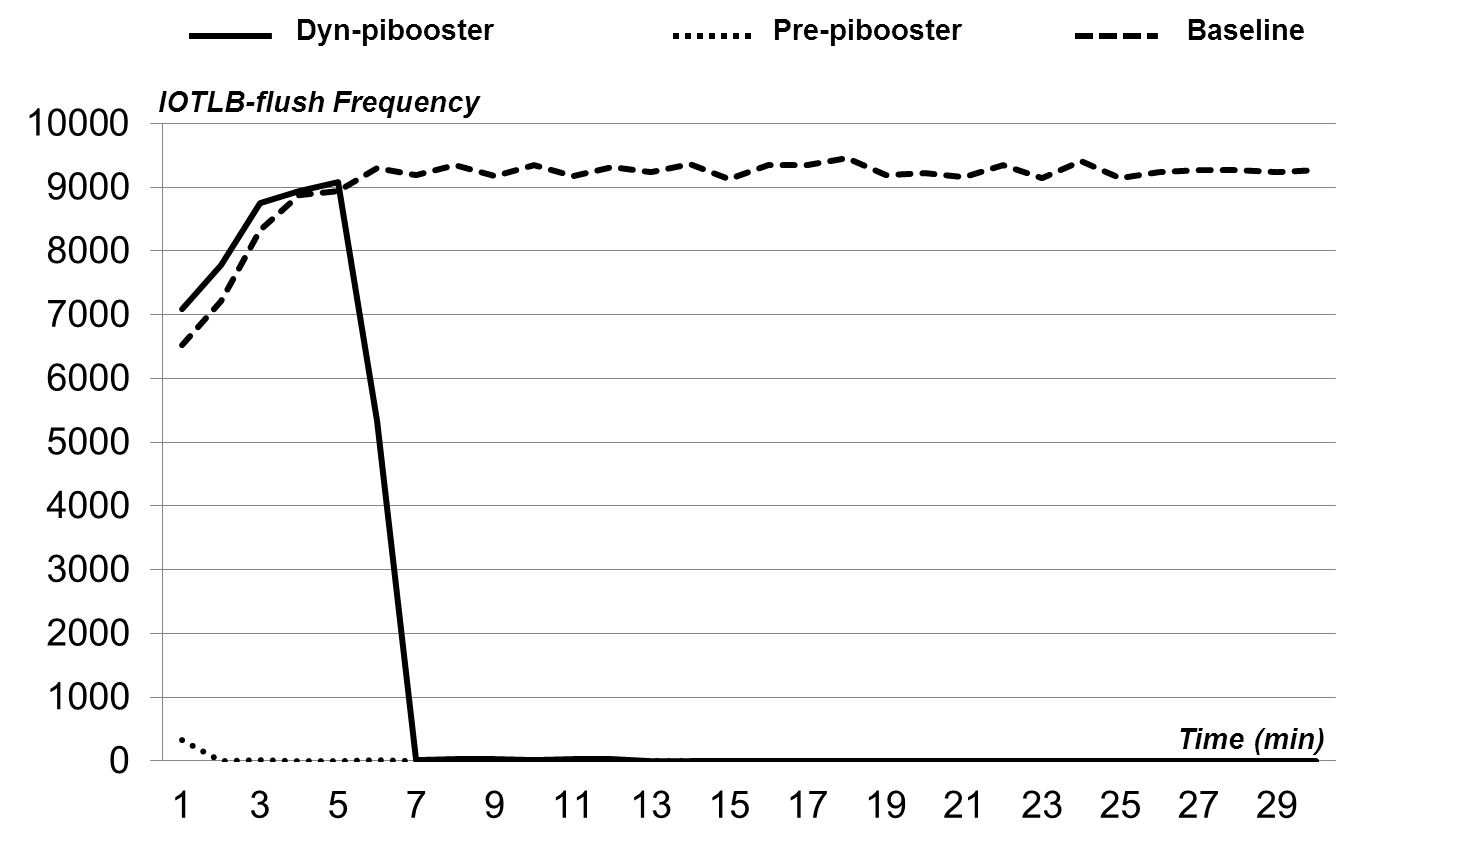
\includegraphics[scale=0.55]{image/iotlbflush.png} \\
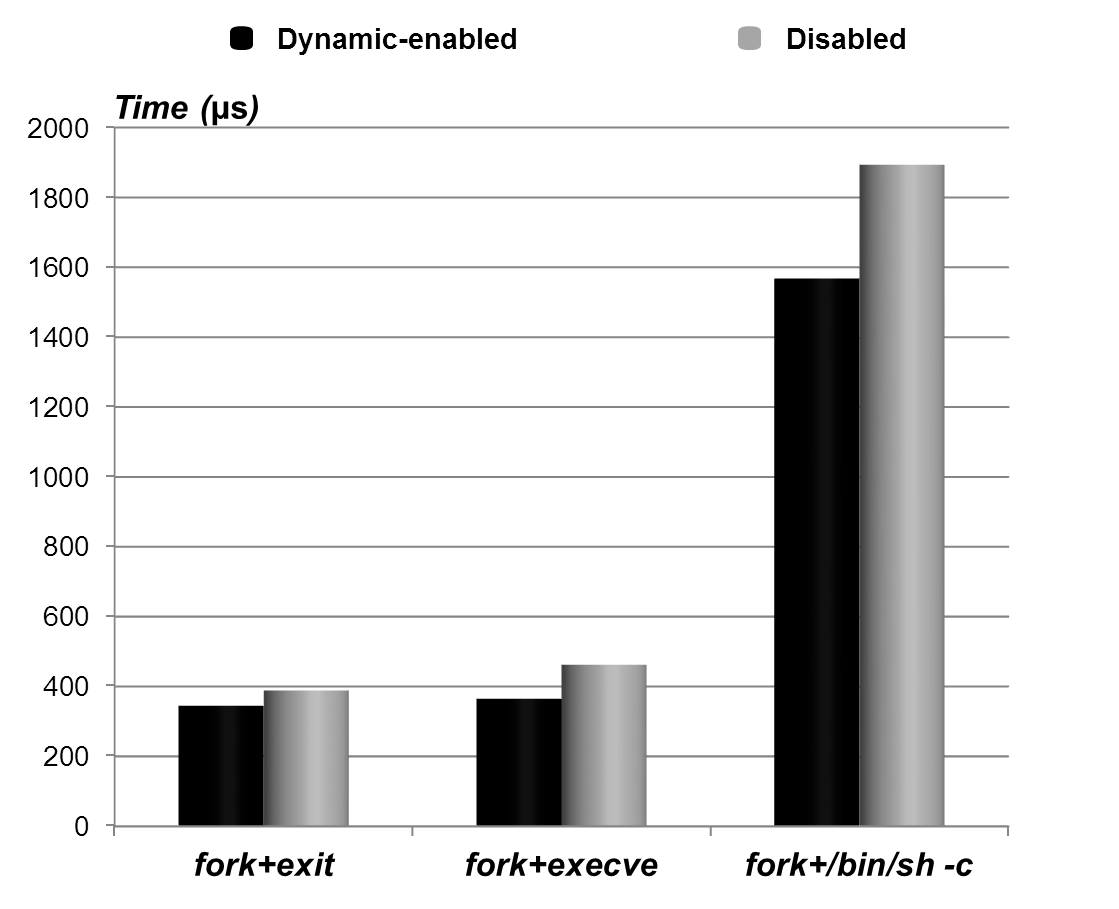
\includegraphics[width=0.5\textwidth]{image/macro/lmbench.png} \\
\caption{The execution time of all processes in the dyn-\name group is reduced by 24\%, compared to that of the baseline group.}
\label{fig:lmbench}
\end{figure}

Lmbench is used to measure CPU time that processes cost (i.e., fork+exit, fork+execve, fork+/bin/sh -c), shown in Figure~\ref{fig:lmbench}. The configuration parameters are selected by default, except parameters of processor MHz, a range of memory and mail result, since CPU mhz of our test machine is $3.2$ GHz rather than the default one, memory range uses $1024$ MB to save time cost of one Lmbench-run and we need no results mailed. As can be seen from the figure, the processes of fork+exit, fork+execve and fork+/bin/sh -c in the dyn-\name group costs $344$, $365$, and $1567$ in microseconds, $11$\%, $17$\%, $21$\% fewer than that of the baseline group. Undoubtedly, \name has improved CPU performance.

\begin{figure}[htp]
\centering
%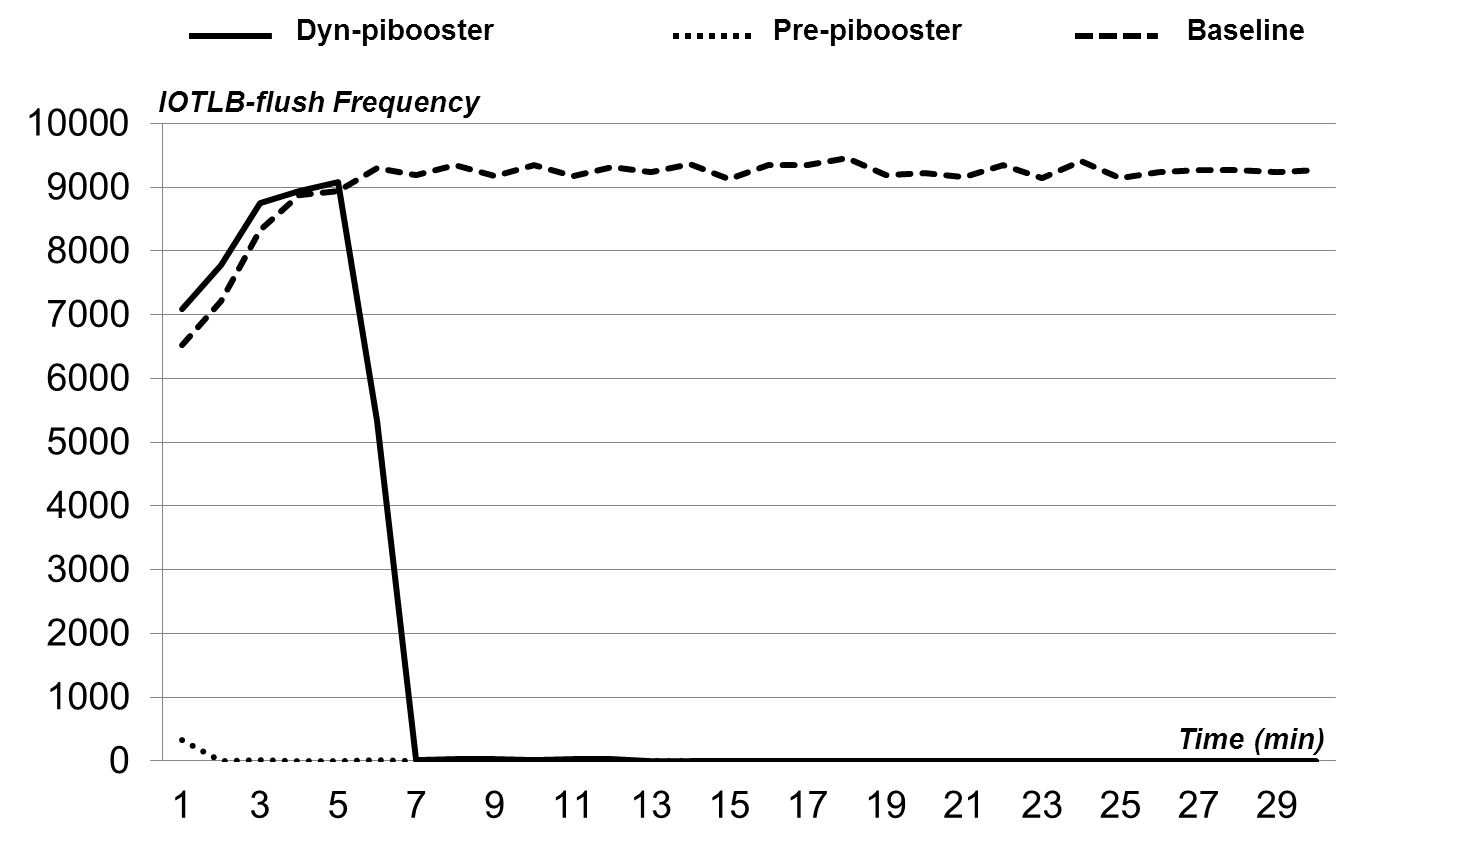
\includegraphics[scale=0.55]{image/iotlbflush.png} \\
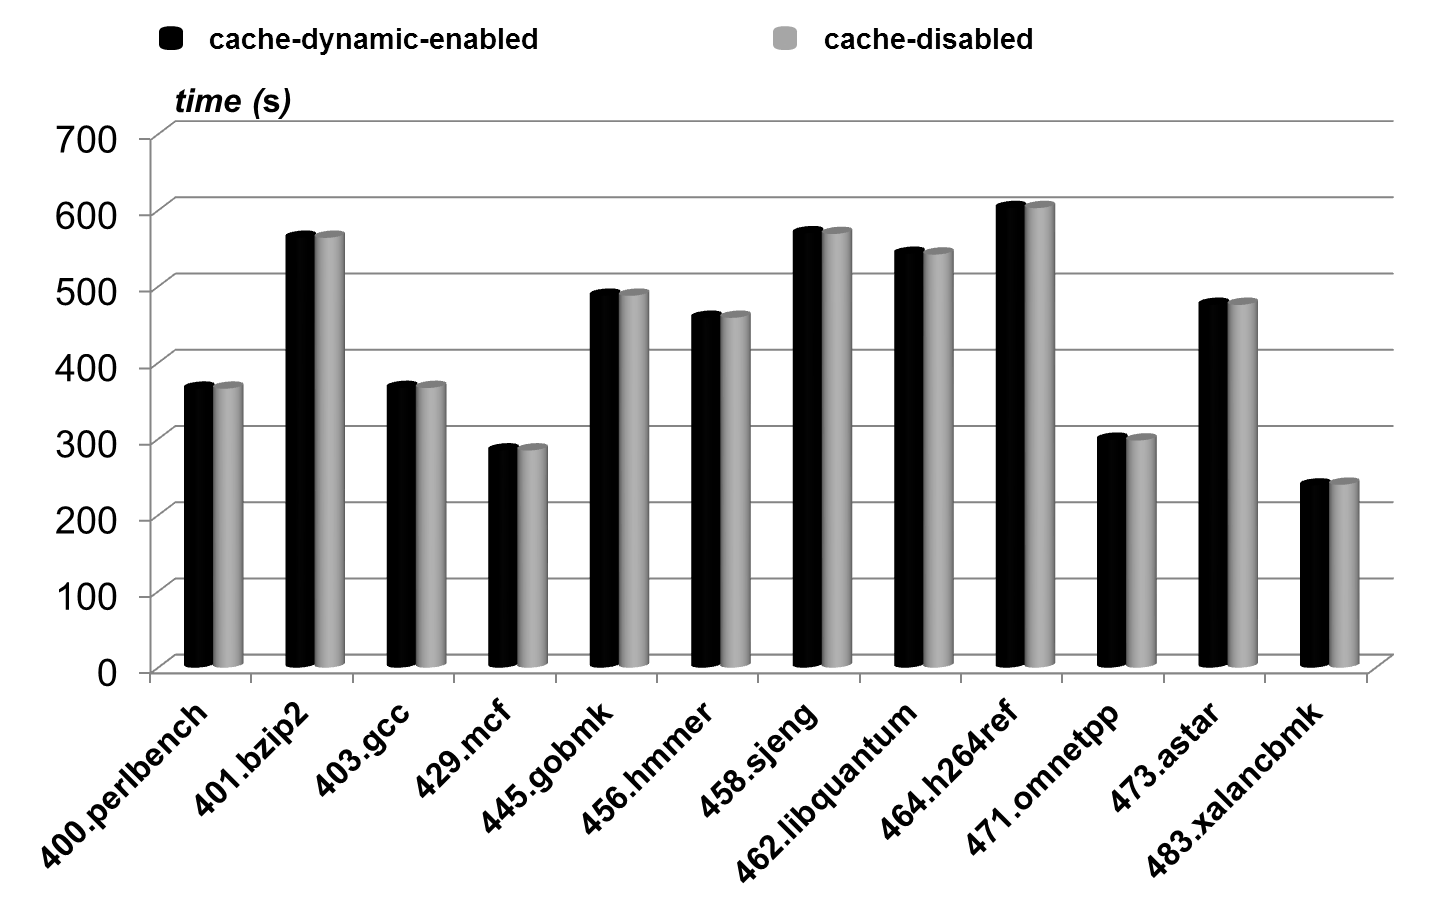
\includegraphics[width=0.5\textwidth]{image/macro/spec.png} \\
\caption{the maximum difference among all the benchmarks is within 0.42\%, indicating that system performance produced by \name is almost the same as the baseline.}
\label{fig:spec}
\end{figure}

SPECint\_2006v1.2 has $12$ benchmarks in total and they are all invoked with EXAMPLE-linux64-ia32-gcc43+.cfg for integer computation, results of which produce Figure~\ref{fig:spec}. Among the benchmarks, the time costs between the two groups vary little and the maximum difference is within 0.42\%, which is produced by the 483.xalancbmk. In the dyn-\name group it costs $239$ seconds, 0.42\% fewer than that of the baseline group, which poses . Thus, the little difference between the two groups indicates that \name does not impose any bad effect on system performance.



%\begin{figure}[htp]
%\centering
%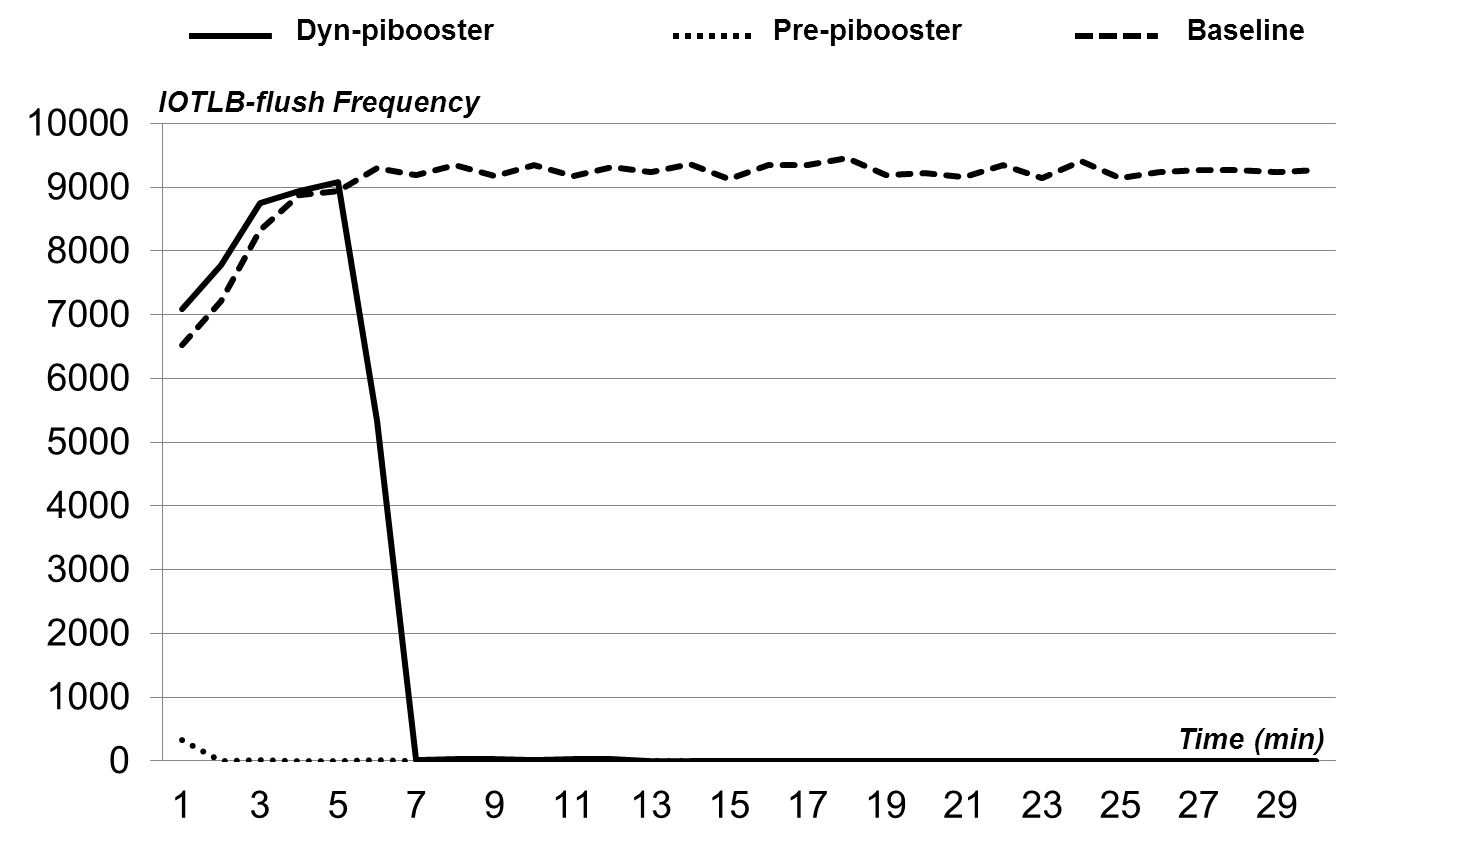
\includegraphics[scale=0.55]{image/iotlbflush.png} \\
%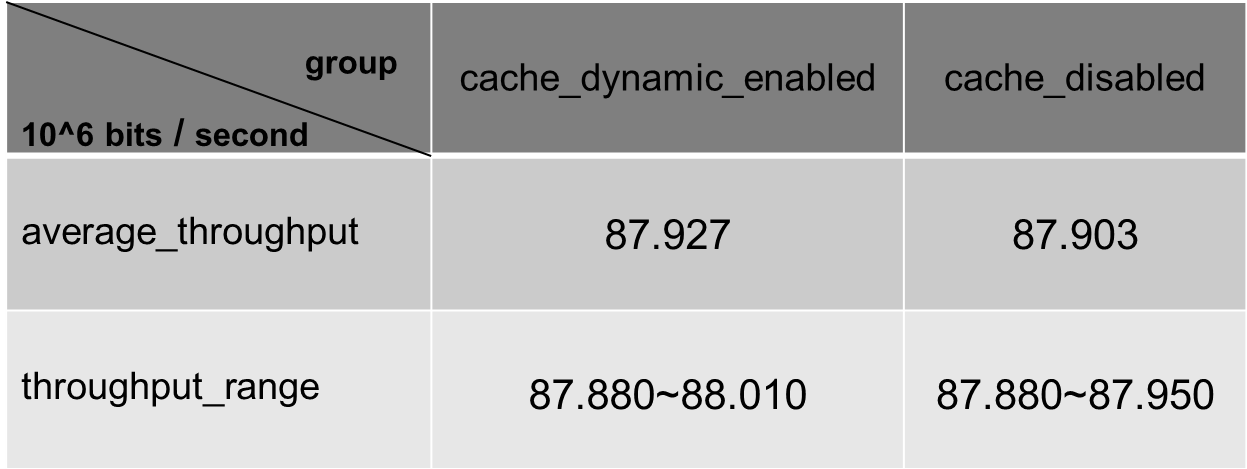
\includegraphics[width=0.5\textwidth]{image/macro/netperf.png} \\
%\caption{Netperf}
%\label{fig:netperf}
%\end{figure}
%|p{1.7cm}|p{1.8cm}|p{1.7cm}


%\begin{figure*}[!t]
%\centering
%\subfigure[PGD Alloc]{
%\label{fig:subfig:a}
%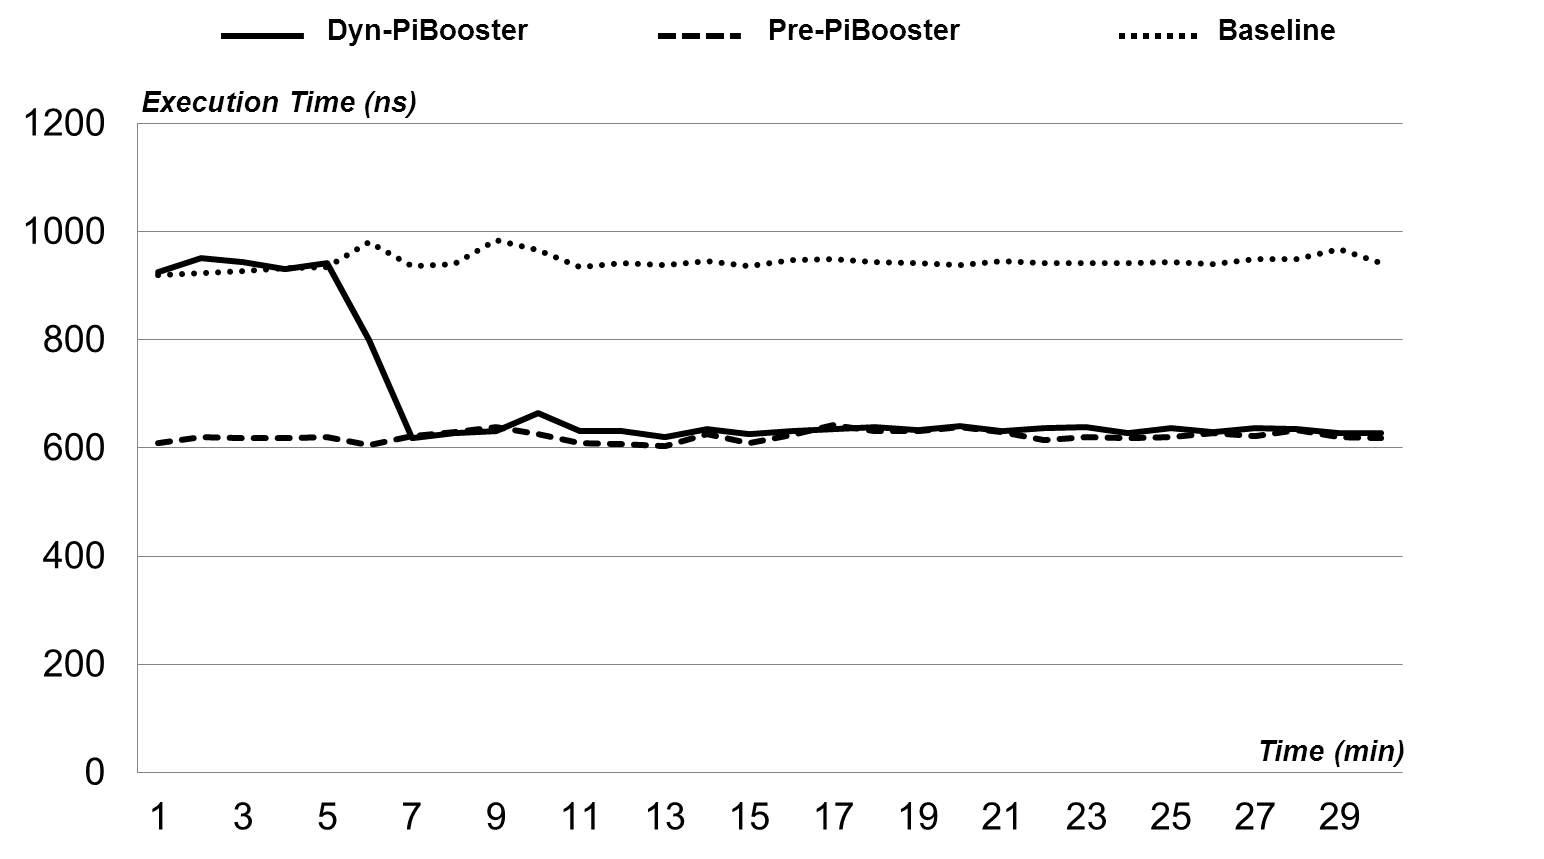
\includegraphics[width=0.5\textwidth]{image/micro/PGDalloc.png}}
%\hspace{1in}
%\subfigure[PGD Free]{
%\label{fig:subfig:b}
%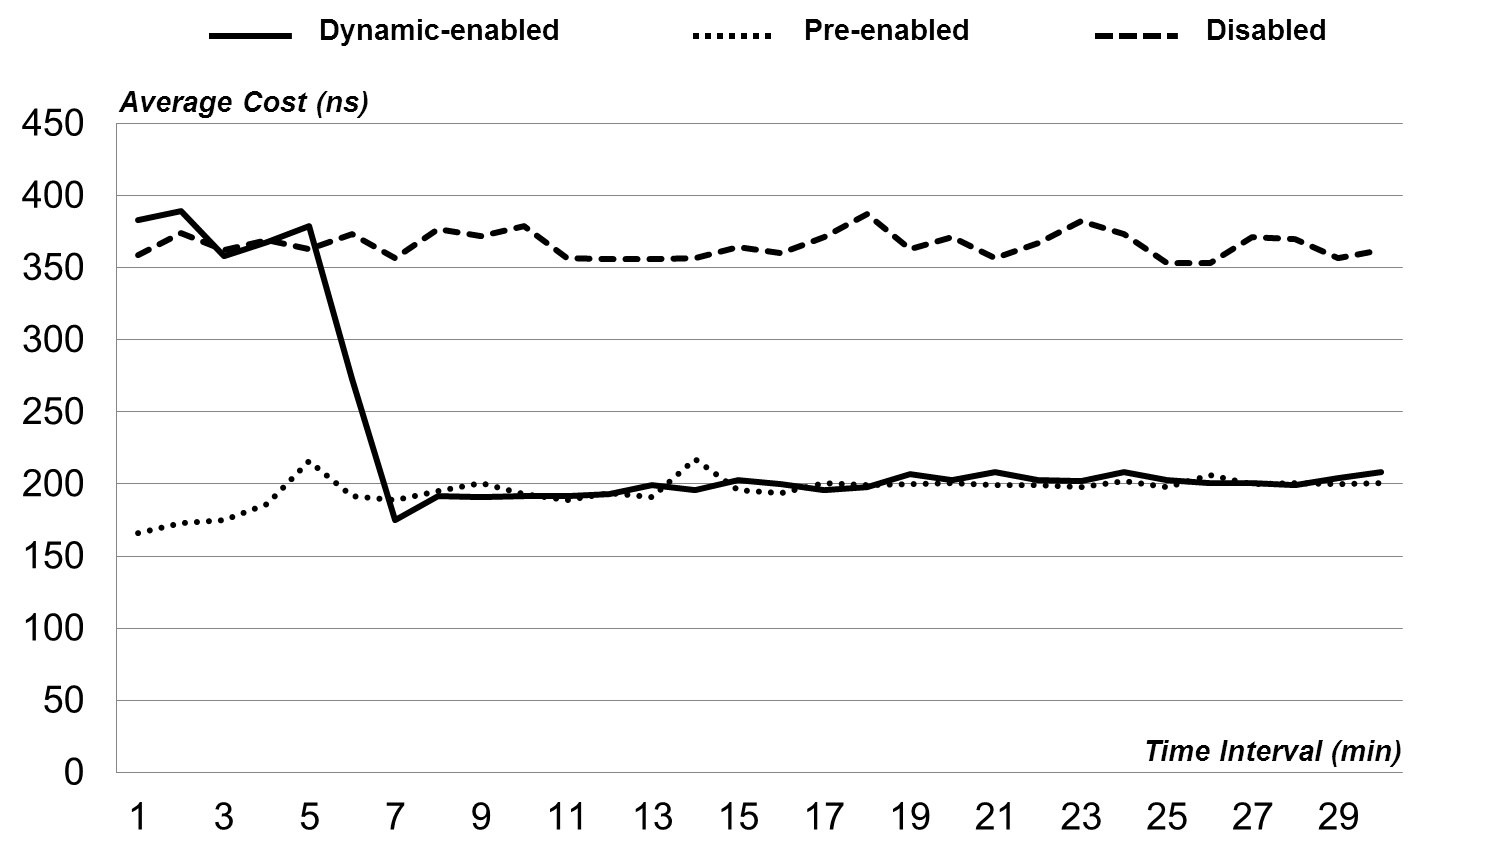
\includegraphics[width=0.5\textwidth]{image/micro/PGDfree.png}}
%\caption{Both page-table cache groups costs much less CPU cycles}
%\label{fig:PGDtime} %% label for entire figure
%\end{figure*}

%\begin{figure}
%\centering
%\subfigure[PGD]{
%\label{fig:subfig:a}
%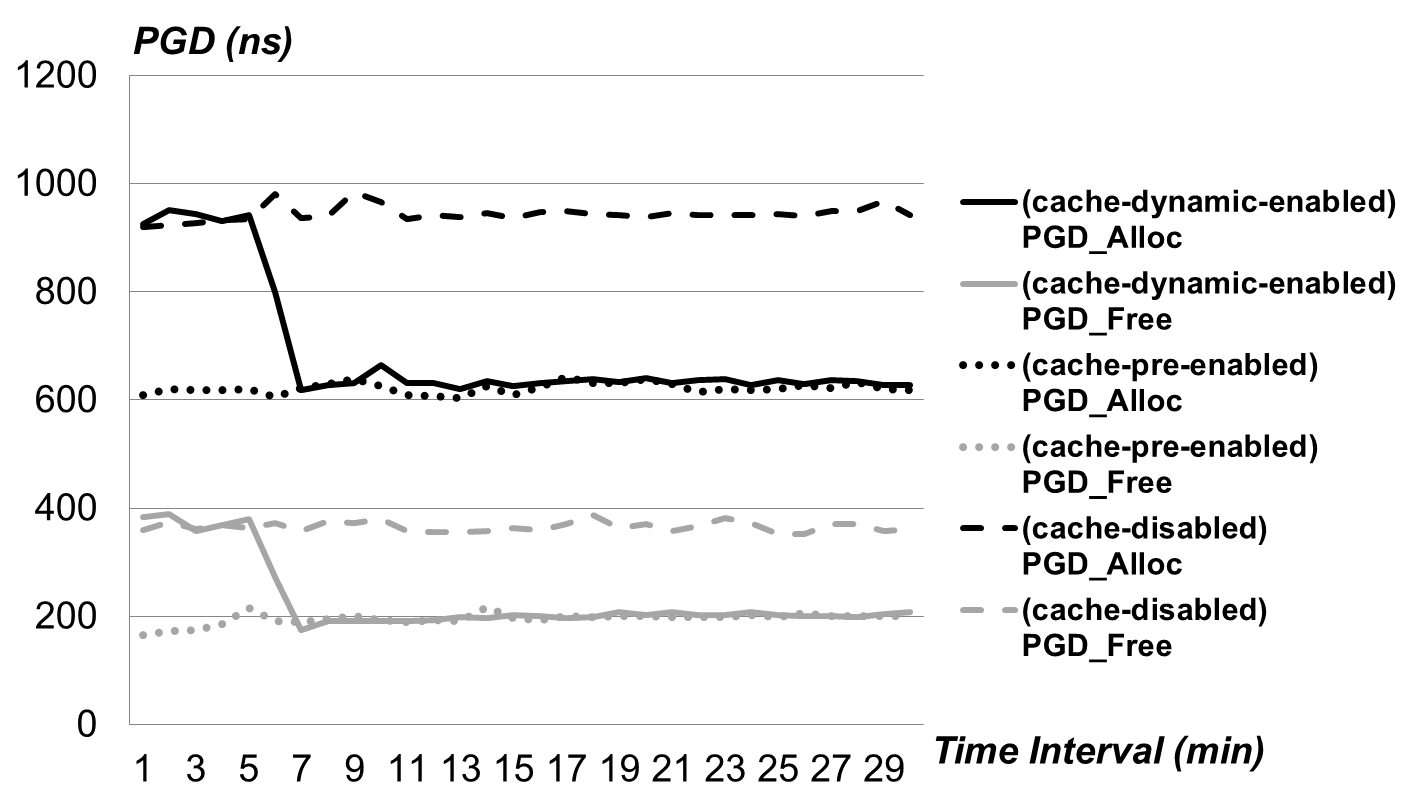
\includegraphics[width=0.5\textwidth]{image/micro/PGDtime.png}}
%\hspace{1in}
%\subfigure[PMD]{
%\label{fig:subfig:b}
%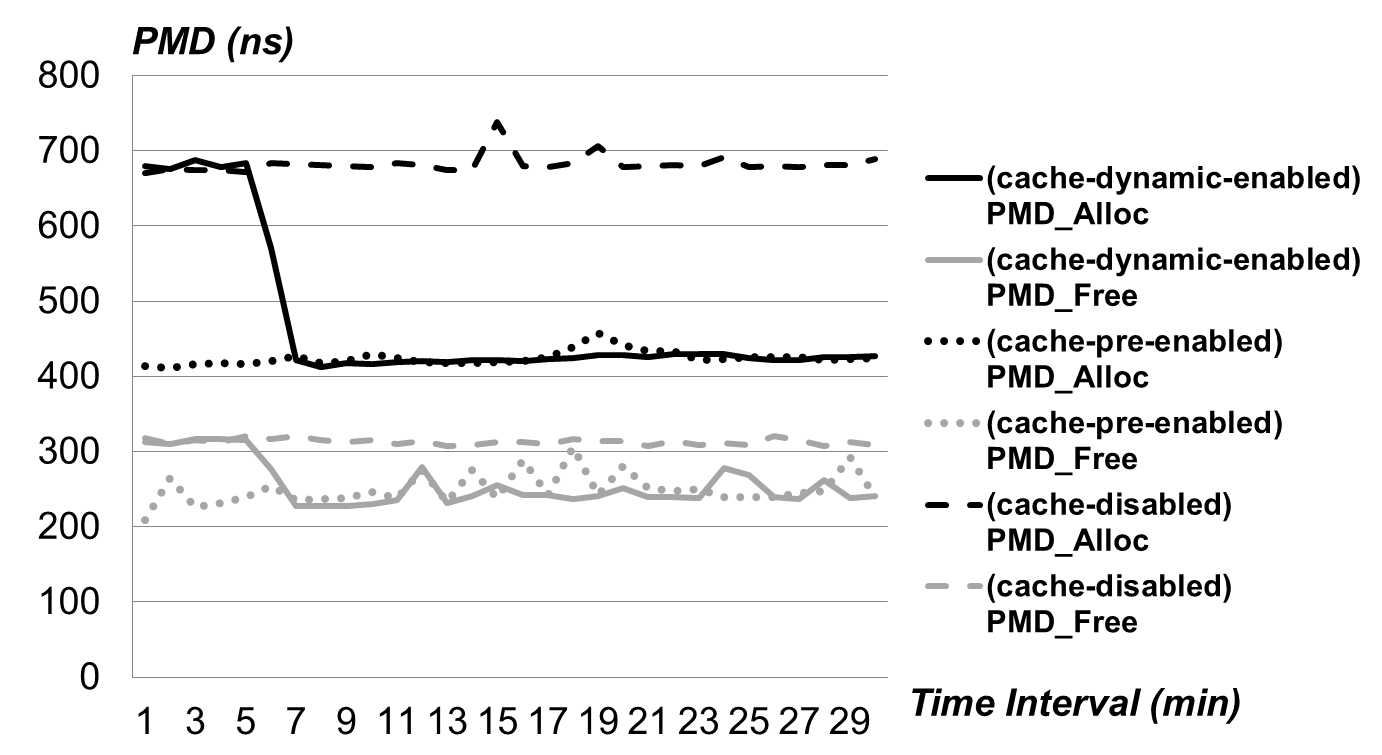
\includegraphics[width=0.5\textwidth]{image/micro/PMDtime.png}}
%\hspace{1in}
%\subfigure[PTE]{
%\label{fig:subfig:c}
%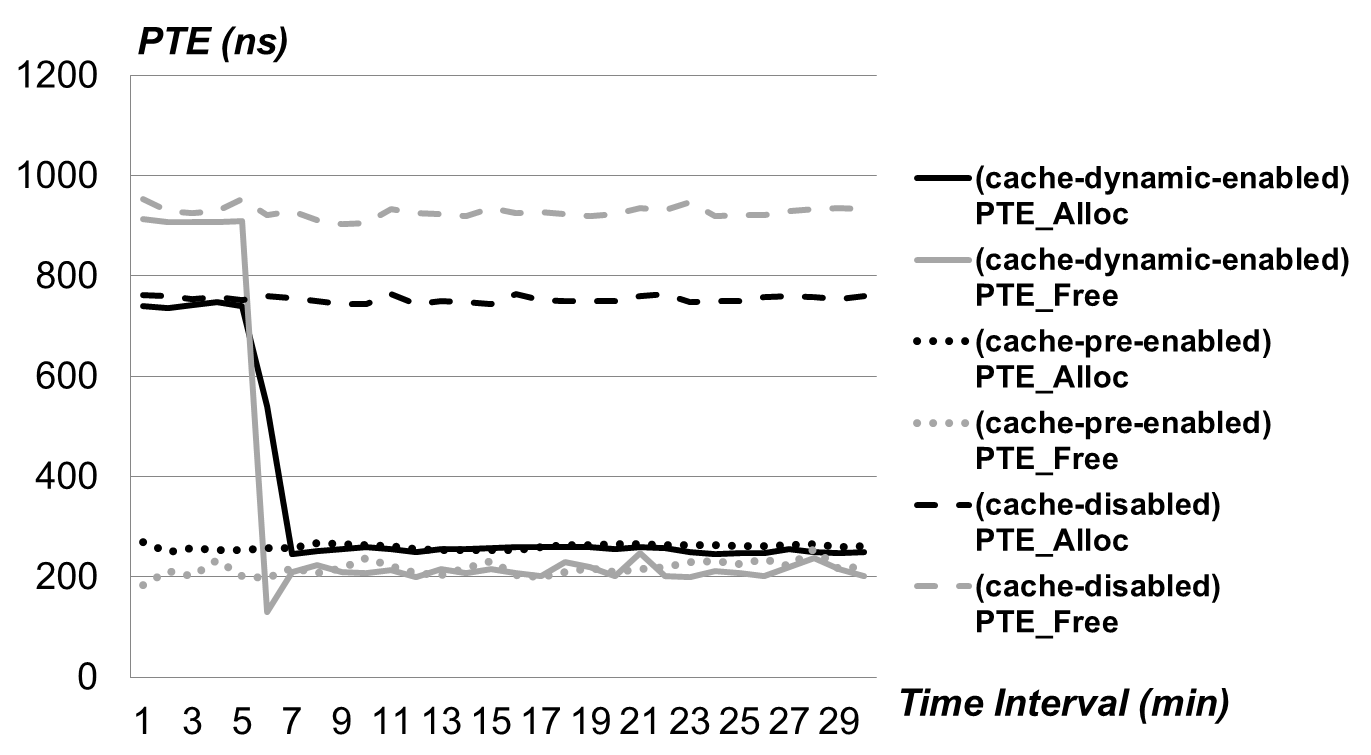
\includegraphics[width=0.5\textwidth]{image/micro/PTEtime.png}}
%\caption{CPU Usage for Each Level of Page Table}
%\label{fig:PGtime} %% label for entire figure
%\end{figure}

%\begin{figure}
%\centering
%\subfigure[PGD]{
%\label{fig:subfig:a}
%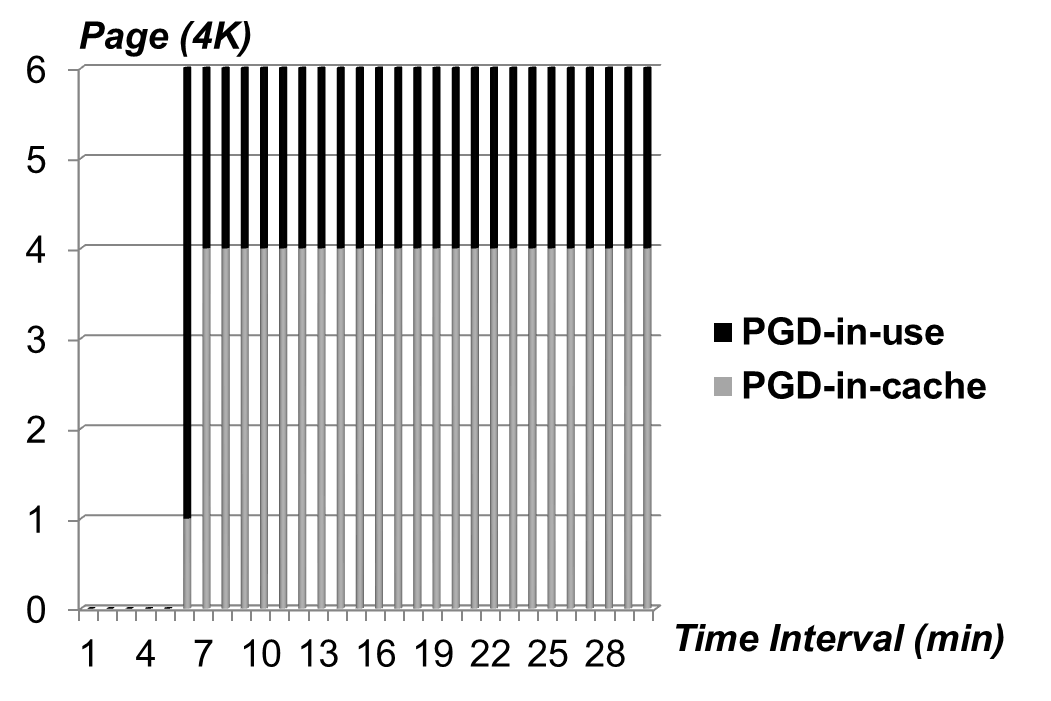
\includegraphics[width=0.5\textwidth]{image/micro/dyn_PGDpool.png}}
%\hspace{1in}
%\subfigure[PMD]{
%\label{fig:subfig:b}
%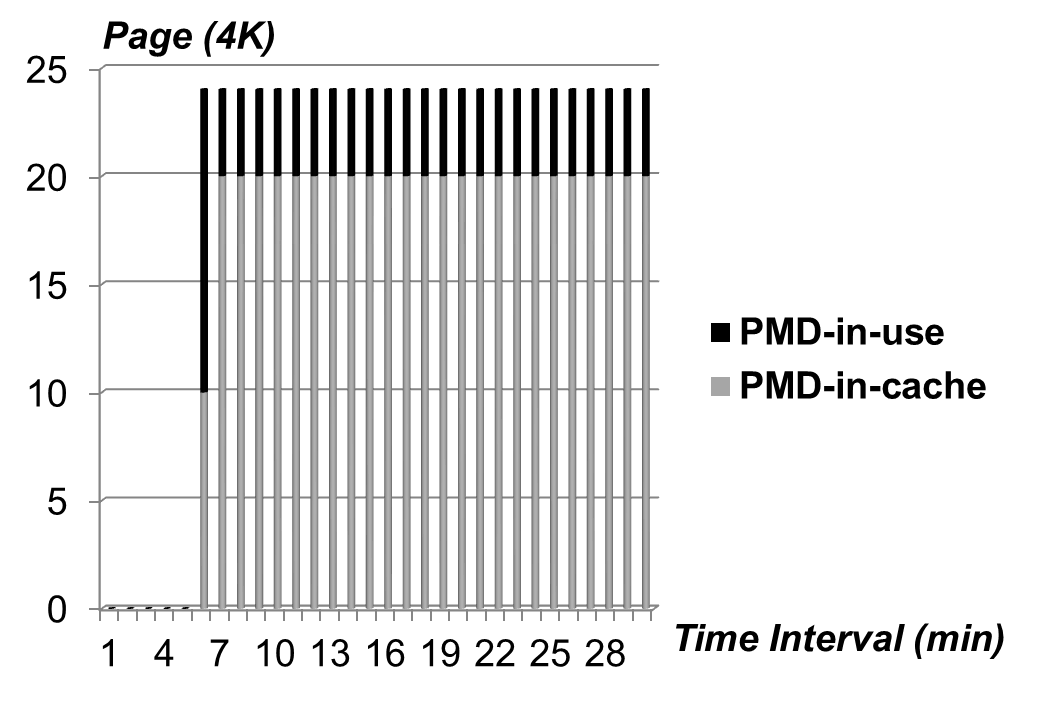
\includegraphics[width=0.5\textwidth]{image/micro/dyn_PMDpool.png}}
%\hspace{1in}
%\subfigure[PTE]{
%\label{fig:subfig:c}
%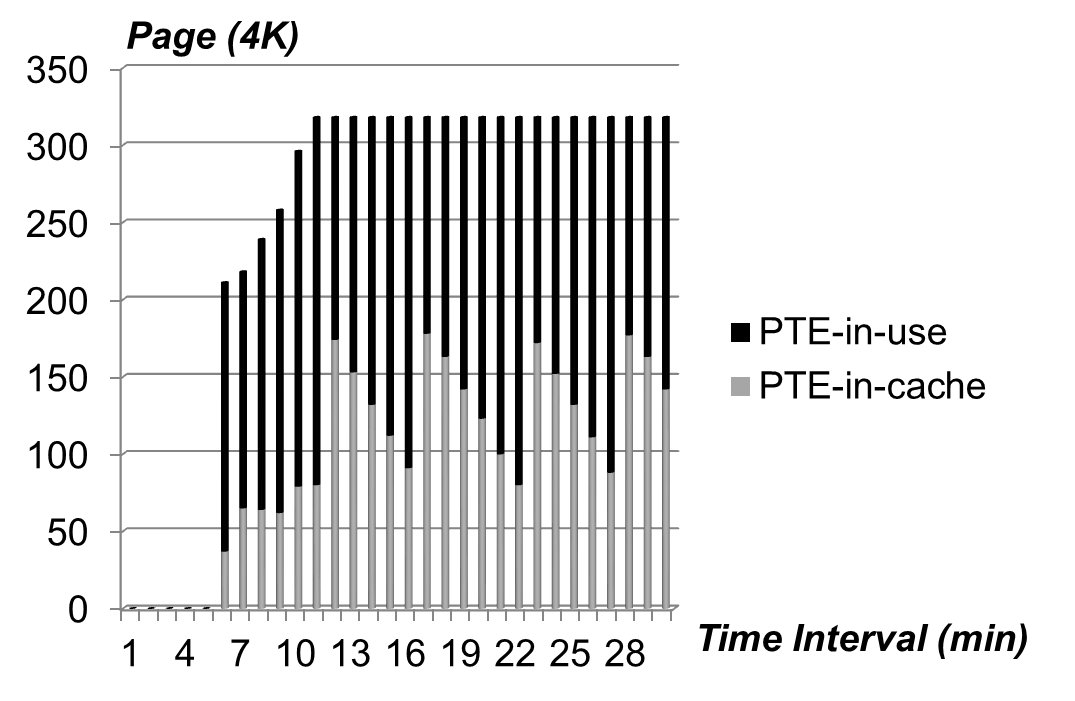
\includegraphics[width=0.5\textwidth]{image/micro/dyn_PTEpool.png}}
%\caption{Cache Pools Size for Cache-Dynamic-Enabled Group}
%\label{fig:dynPGpool} %% label for entire figure
%\end{figure}

%\begin{figure}
%\centering
%\subfigure[PGD]{
%\label{fig:subfig:a}
%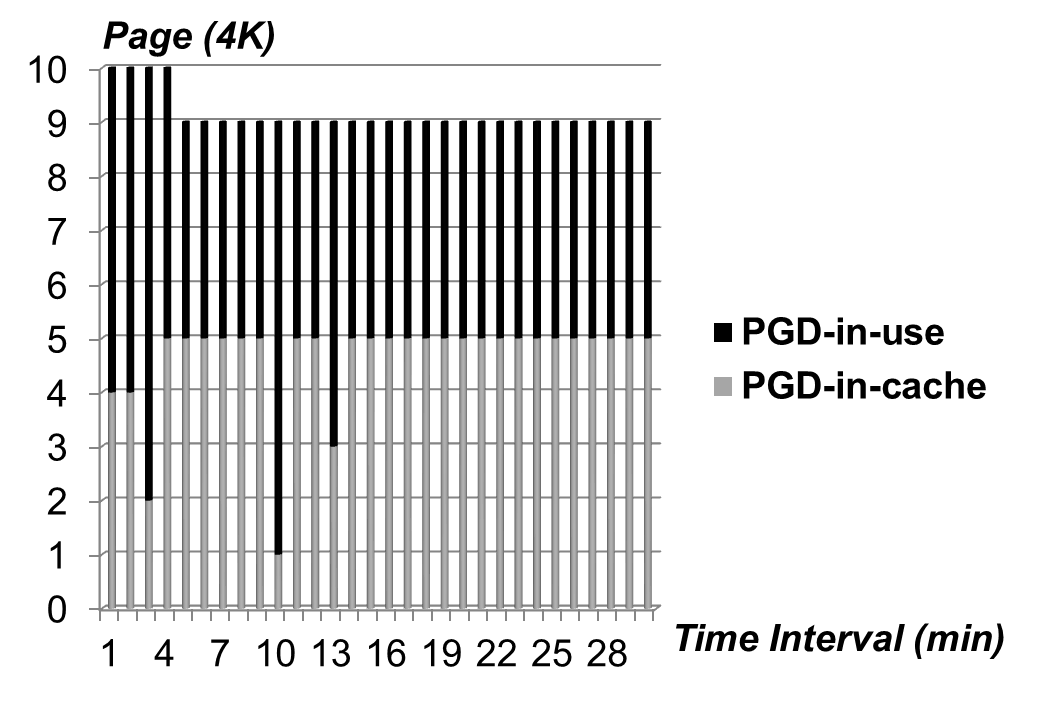
\includegraphics[width=0.5\textwidth]{image/micro/pre_PGDpool.png}}
%\hspace{1in}
%\subfigure[PMD]{
%\label{fig:subfig:b}
%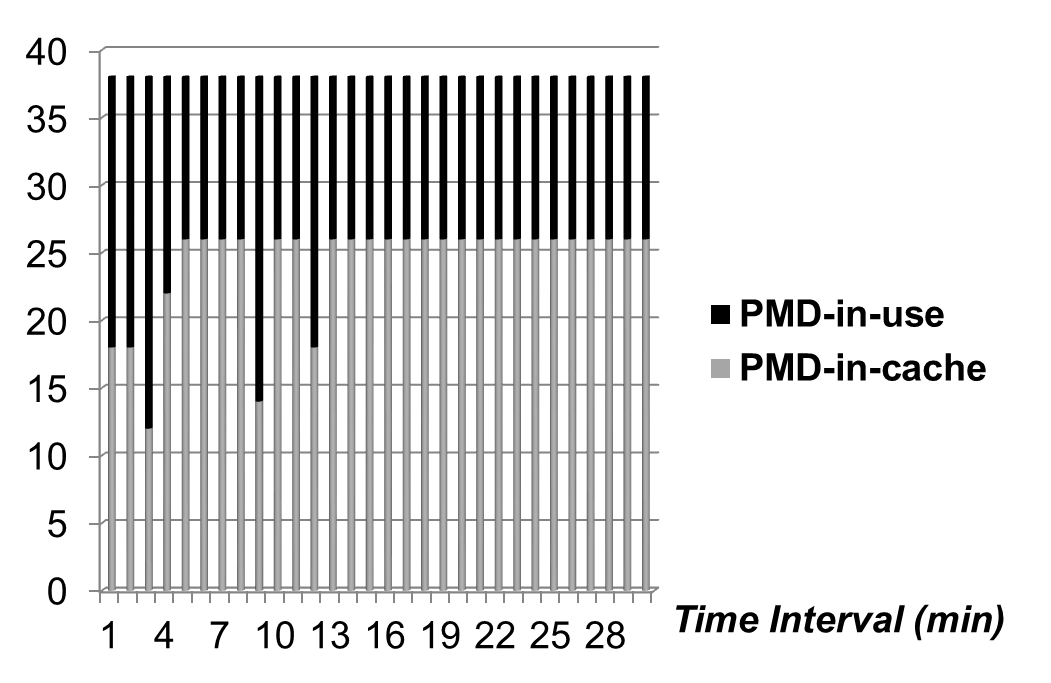
\includegraphics[width=0.5\textwidth]{image/micro/pre_PMDpool.png}}
%\hspace{1in}
%\subfigure[PTE]{
%\label{fig:subfig:c}
%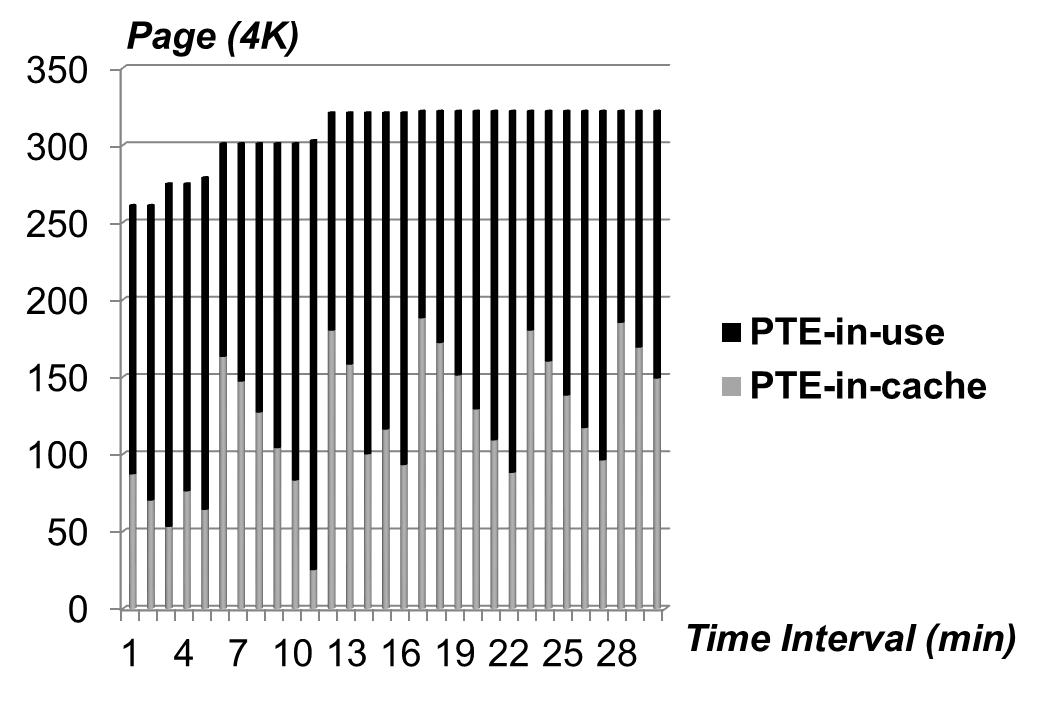
\includegraphics[width=0.5\textwidth]{image/micro/pre_PTEpool.png}}
%\caption{Cache Pools Size for Cache-Pre-Enabled Group}
%\label{fig:prePGpool} %% label for entire figure
%\end{figure}

%PGD & $5$  & $4$   & $>1:1$ \\ \hline
%PMD & $26$ & $12$   & $>2:1$ \\ \hline
%PTE & $145$ & $177$ & $<1:1$ \\ \hline
%Total & $176$ & $193$ & $<1:1$ \\ \hline

%PGD & $4$  & $2$   & $2:1$ \\ \hline
%PMD & $20$ & $4$   & $5:1$ \\ \hline
%PTE & $136$ & $182$ & $<1:1$ \\ \hline
%Total & $160$ & $188$ & $<1:1$ \\ \hline
